\section{Network Architecture}
\label{architecture}
\begin{figure}
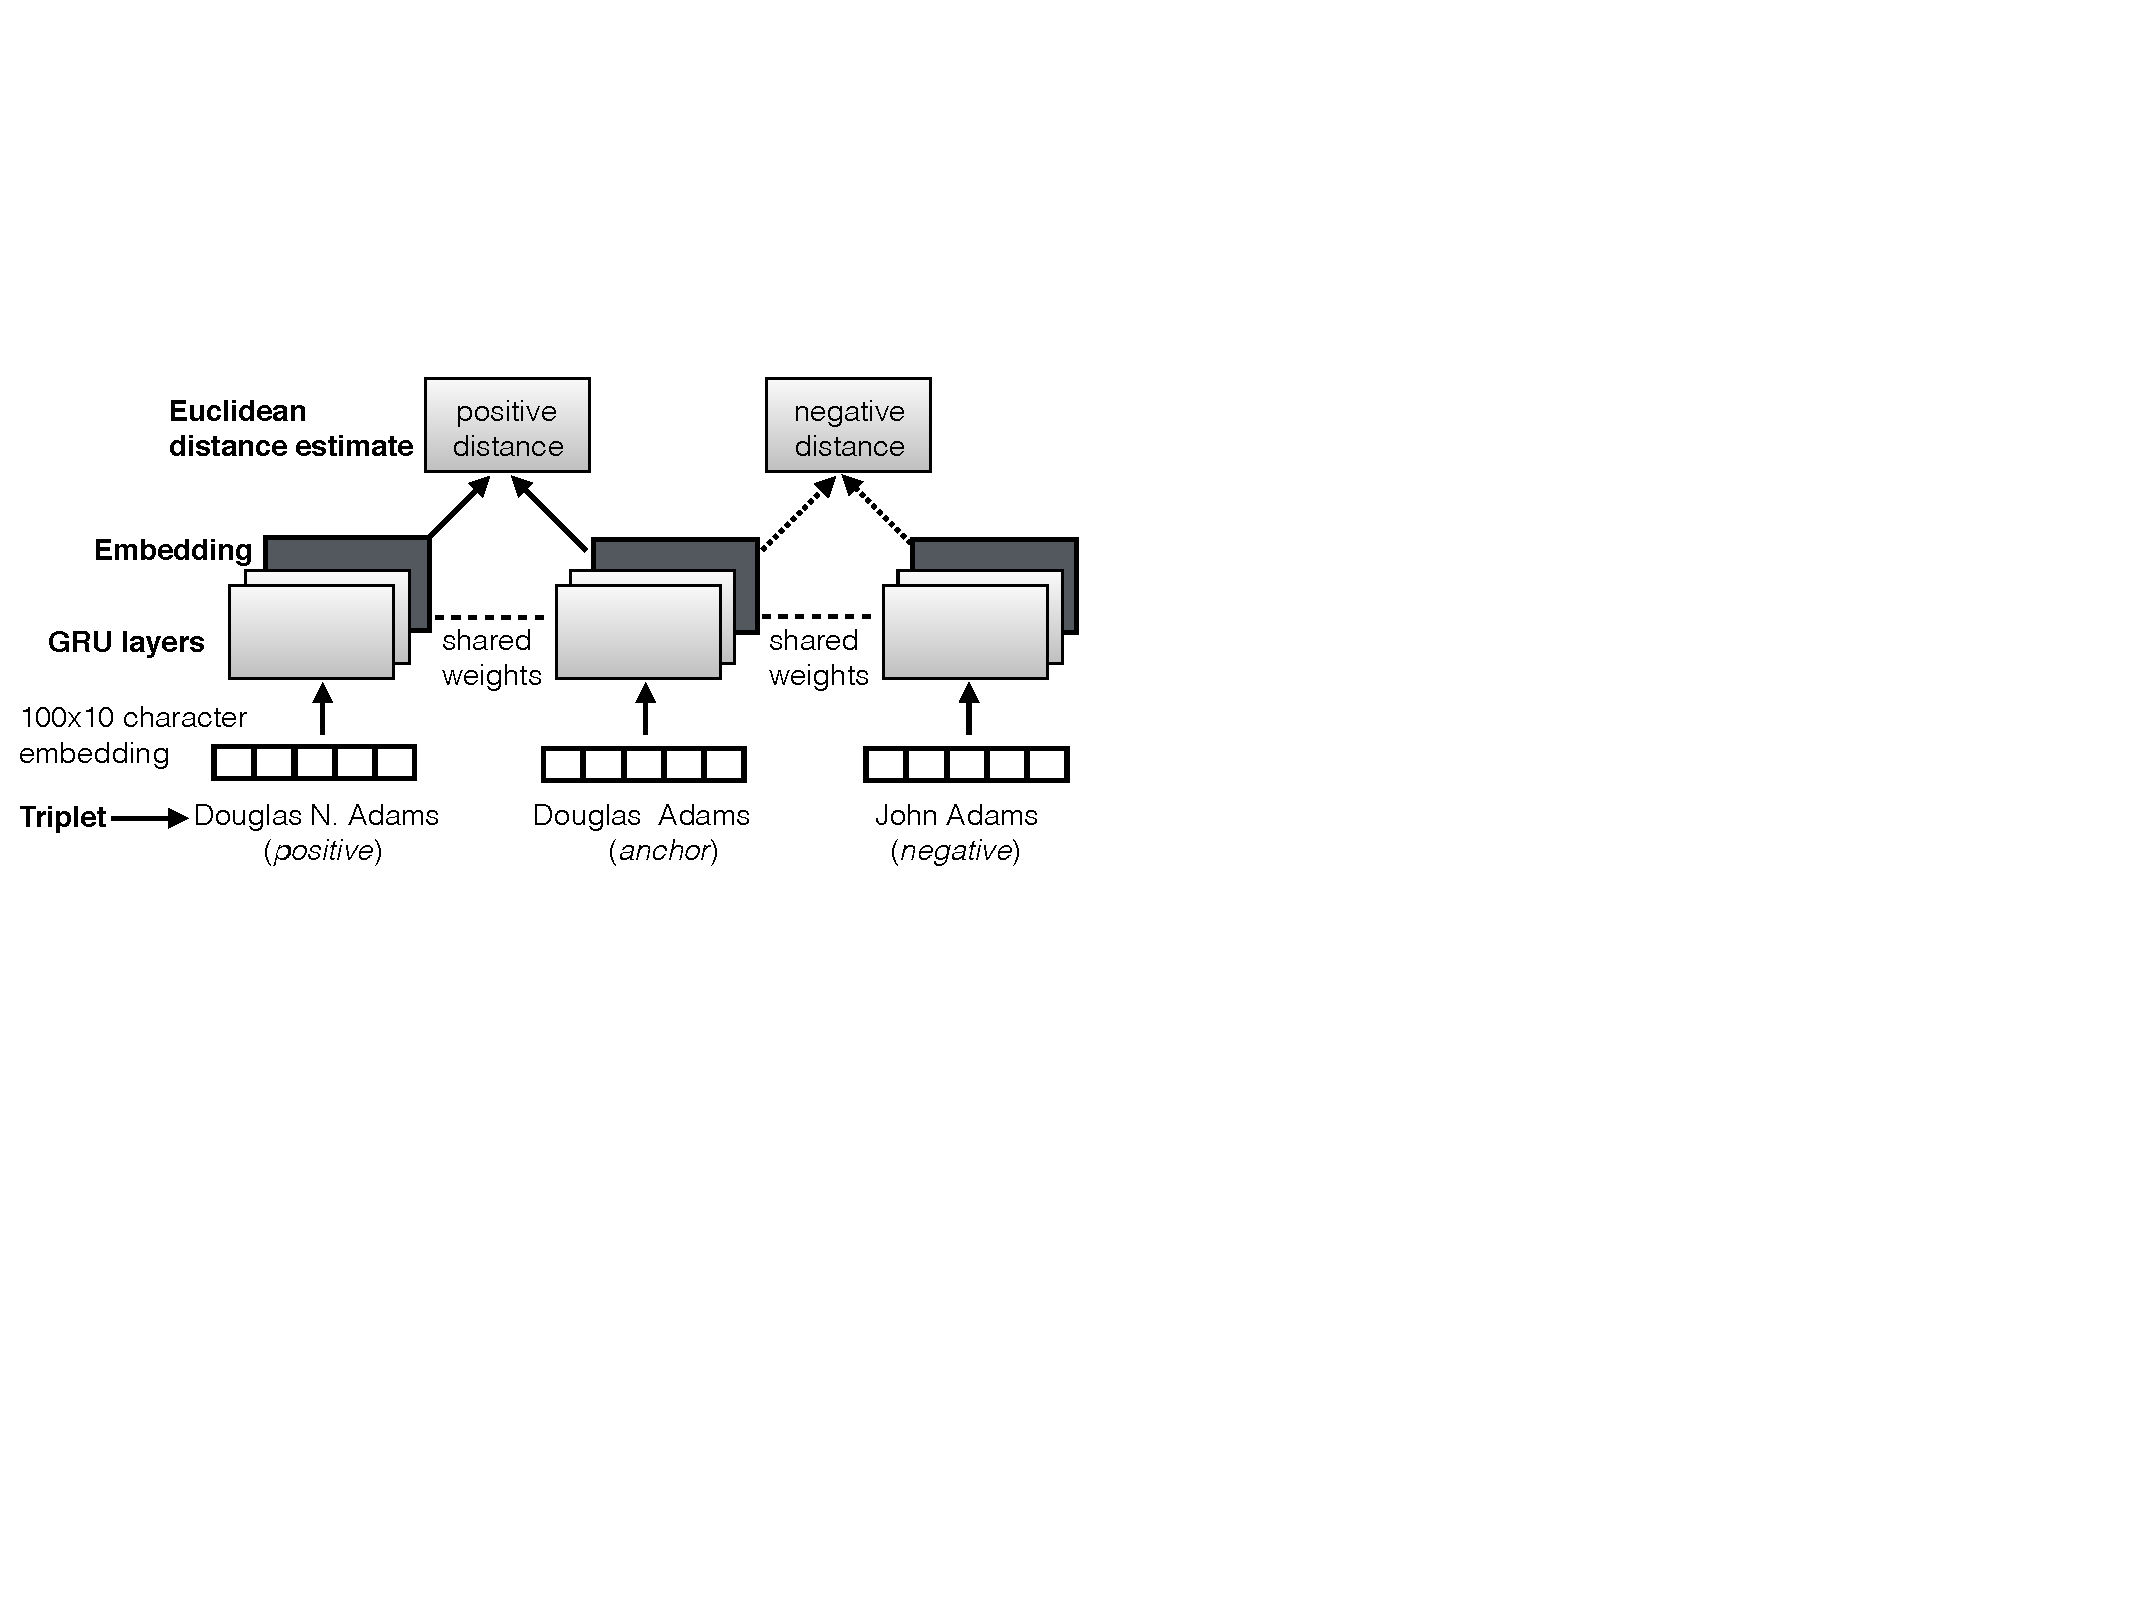
\includegraphics[width=1.0\linewidth]{triplet_siamese_network}
\caption{Architecture of the siamese network}
\label{siamese_nets}
\end{figure}

Figure~\ref{siamese_nets} illustrates the siamese network architecture \cite{DBLP:conf/cvpr/SchroffKP15} we used to build a system for merging data using Keras and Tensorflow.  As stated earlier, input is initially triples of a name, i.e., an \textit{anchor}, a \textit{positive} and a \textit{negative}.  During the tokenization process, we kept punctuation such as `-', `,', and `.' in the name because they are important signals in processing a name.  For the network, input vectors are computed for each entity assuming a maximum name length of 10 for each entity.  A 100 dimensional character embedding was computed for each token in the entity using pretrained character embeddings \cite{hashimoto-jmt:2017:EMNLP2017}, which resulted in a 100 x 10 character encoding for each name used in a triplet.  We used character rather than word embeddings primarily because many names were missing from word based vector embeddings.

These three input character embedding vectors were fed to three identical networks that share the same weights.  Weight sharing ensures that the networks learn the same mapping function.  In our implementation, each of the three networks had 4 stacked layers of 128 unit Gated Recurrent Units (or GRUs) to capture the sequential nature of the input.  For name and textual data, positional information is critical, so we used GRUs instead of the convolutional neural networks (CNNs) that have been traditionally used in metric learning for face and image recognition. GRUs are a type of recurrent network \cite{cho-al-emnlp14} where each hidden unit updates its weights at a specific step in the sequence $t$ based on the current input $x_t$ and the value of the hidden unit from the prior step $h_{t-1}$.  

%$r_t$ is a reset gate which determines whether the state from the previous step $h_{t-1}$ should be ignored. $z_t$ is an update gate which determines whether the current hidden state should be updated with the new hidden state $\tilde{h_t}$.  Equations~\ref{eq_1}-\ref{eq_4} that govern the update at $h_t$, as summarized by \cite{colah}.
%\begin{equation}
%z_t = \sigma(W_z . [h_{t-1}, x_t])
%@\label{eq_1}
%\end{equation}

%\begin{equation}
%r_t = \sigma(W_r . [h_{t-1}, x_t])
%\label{eq_2}
%\end{equation}

%\begin{equation}
%\tilde{h_t} = tanh (W . [r_t * h_{t-1}, x_t])
%\label{eq_3}
%\end{equation}

%\begin{equation}
%h_t = (1- z_t) * h_{t-1} + z_t * \tilde{h_t}
%\label{eq_4}
%\end{equation}

The output of the last layer shown in the Figure~\ref{siamese_nets} as a dark layer is the vector embedding for the inputs.  These are fed to two layers which compute a euclidean distance between the \textit{anchor} and the \textit{positive} (\textit{positive distance}), and the \textit{anchor} and the \textit{negative} (\textit{negative distance}).  Conceptually, there are two objectives in metric learning, one to minimize \textit{positive distances}, and the other to maximize \textit{negative distances}.  As described below, this dual objective can be achieved by different loss functions.  We restrict ourselves to a discussion of the some of the more popular loss functions that are local in nature (i.e., they only look at a single triple).  

\section{Loss functions}
\label{loss_functions}

Let $\mathbf{x}$ represent an embedding for an entity name, and $\bf{x_{a}}$, $\bf{x_{p}}$, $\bf{x_{n}}$ reflect the vector embeddings of the \textit{anchor}, \textit{positive} and \textit{negative}, respectively.  We investigated four different loss functions, three of which have been used in prior literature to explore their effectiveness for the entity metric learning problem.

\begin{figure}[htb]
    \centering
    \begin{subfigure}[t]{0.3\linewidth}
        \centering
        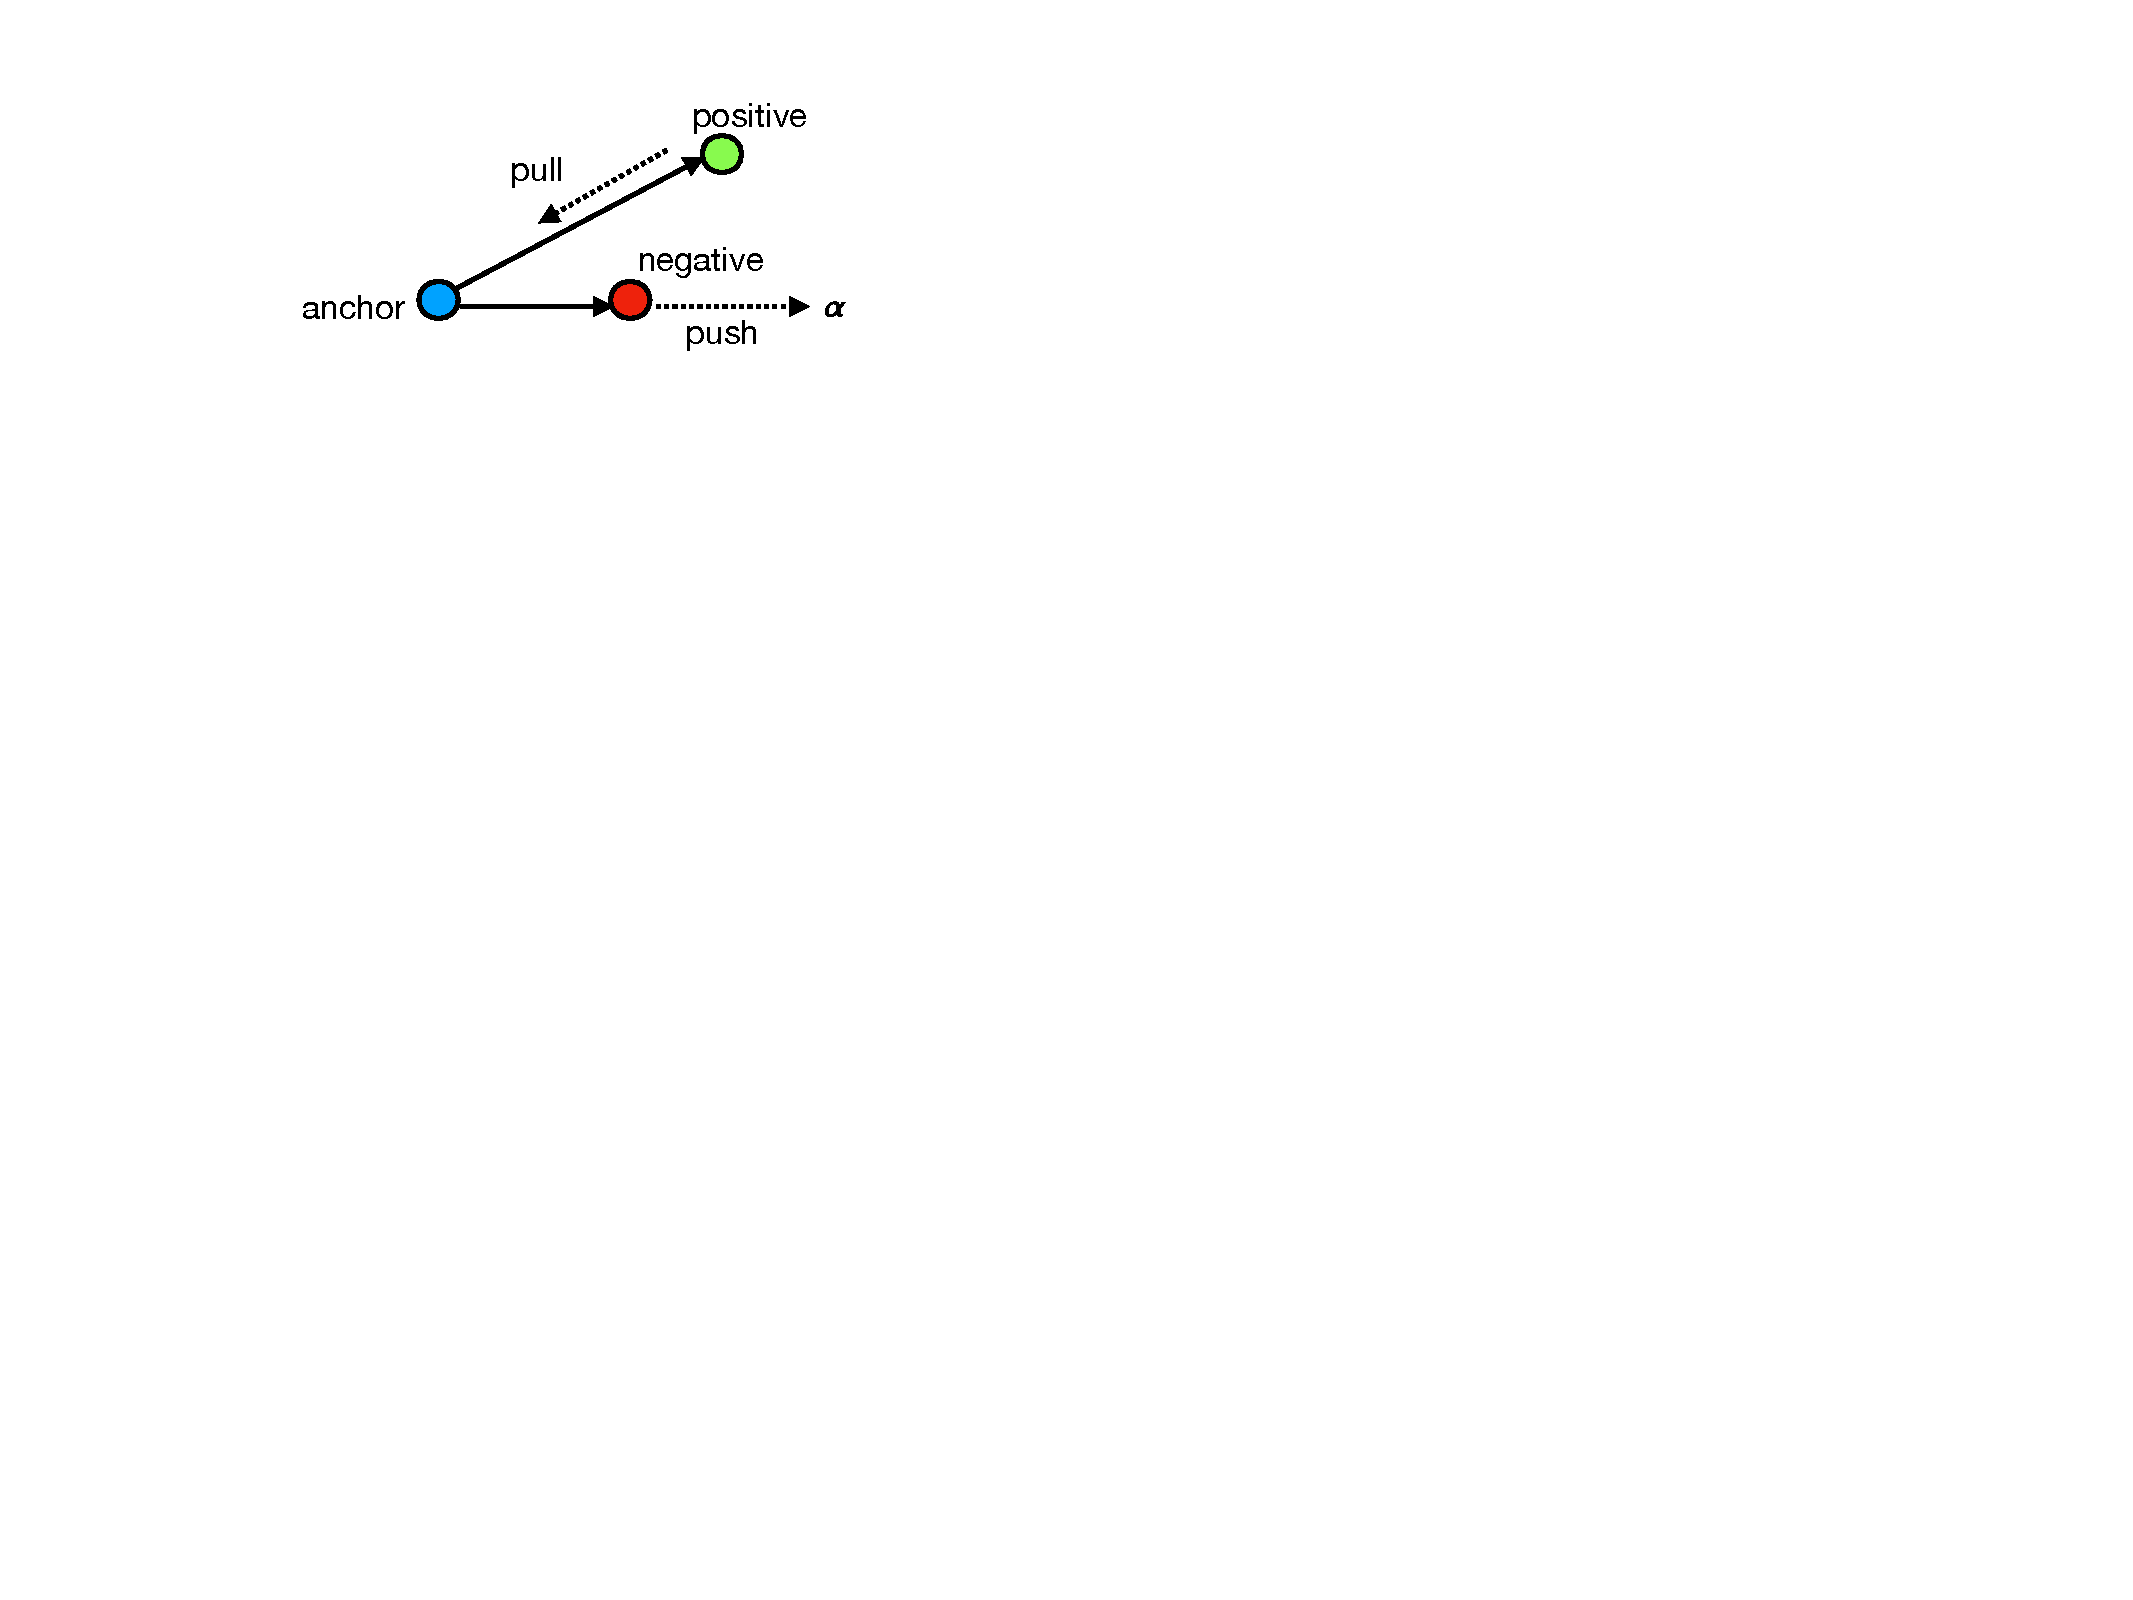
\includegraphics[width=.95\linewidth]{schroff_triplet}
        \caption{Triplet loss}
        \label{schroff_loss}
    \end{subfigure}%
    ~ 
    \begin{subfigure}[t]{0.3\linewidth}
        \centering 
        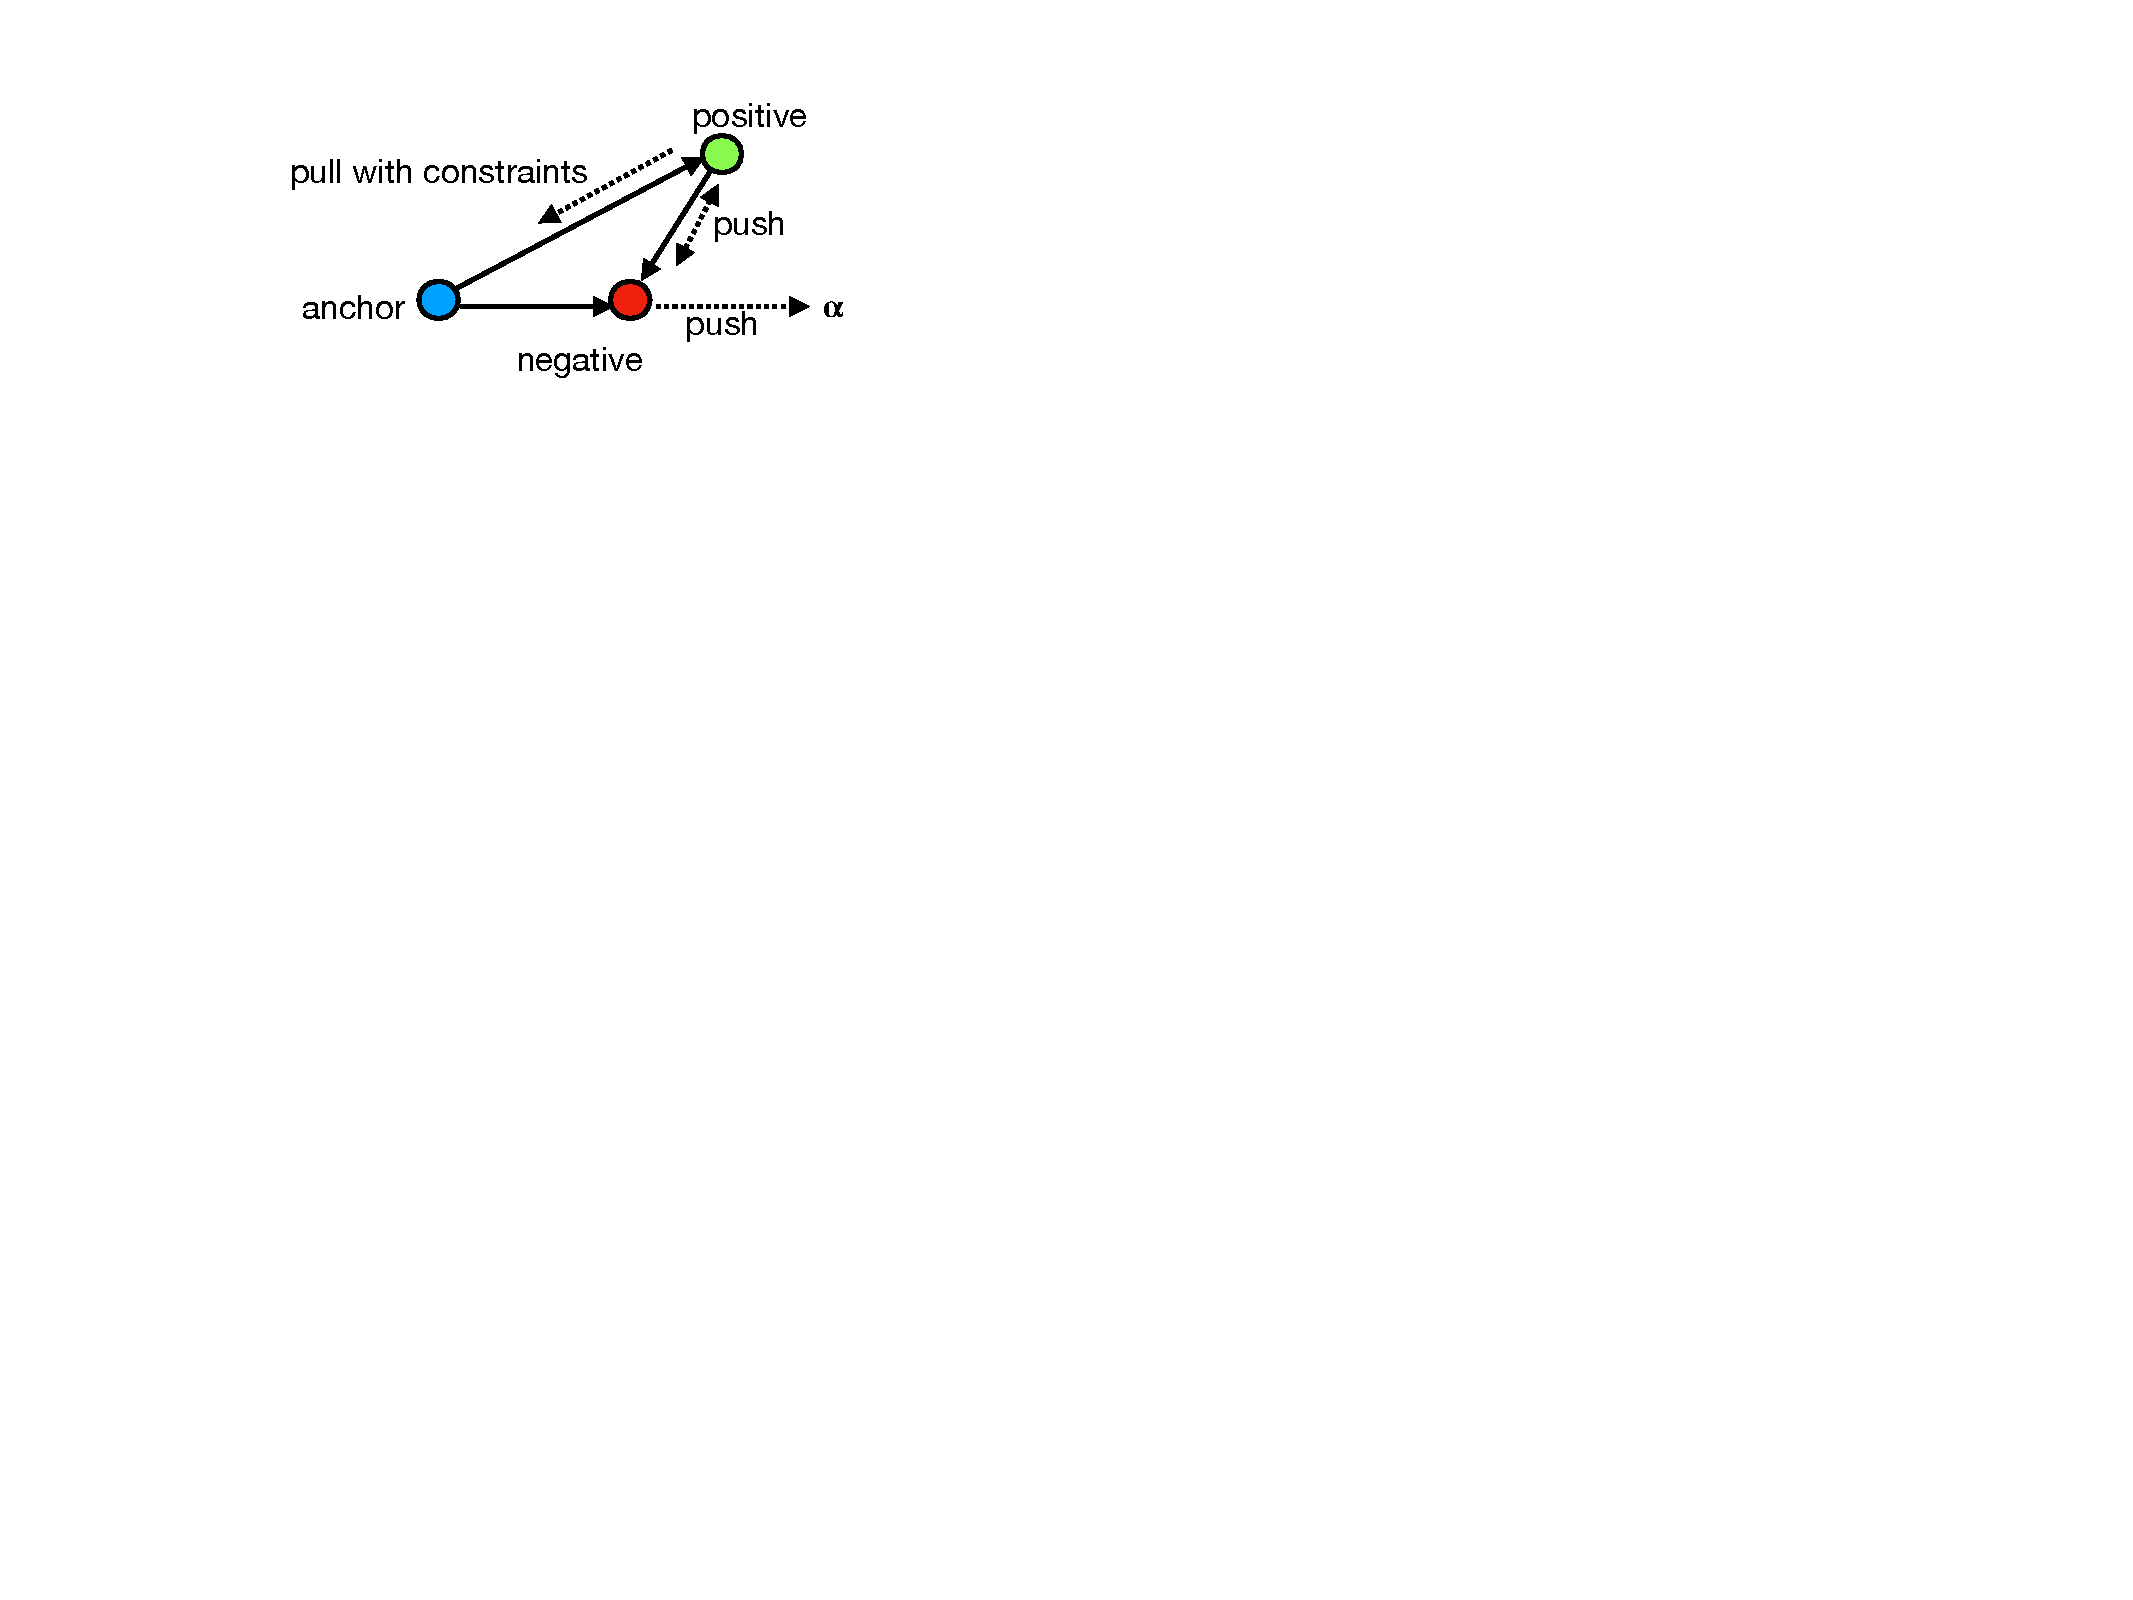
\includegraphics[width=.95\linewidth]{modified_loss}
        \caption{Modified loss}
        \label{modified_loss}
    \end{subfigure}
    ~ 
    \begin{subfigure}[t]{0.3\linewidth}
        \centering 
        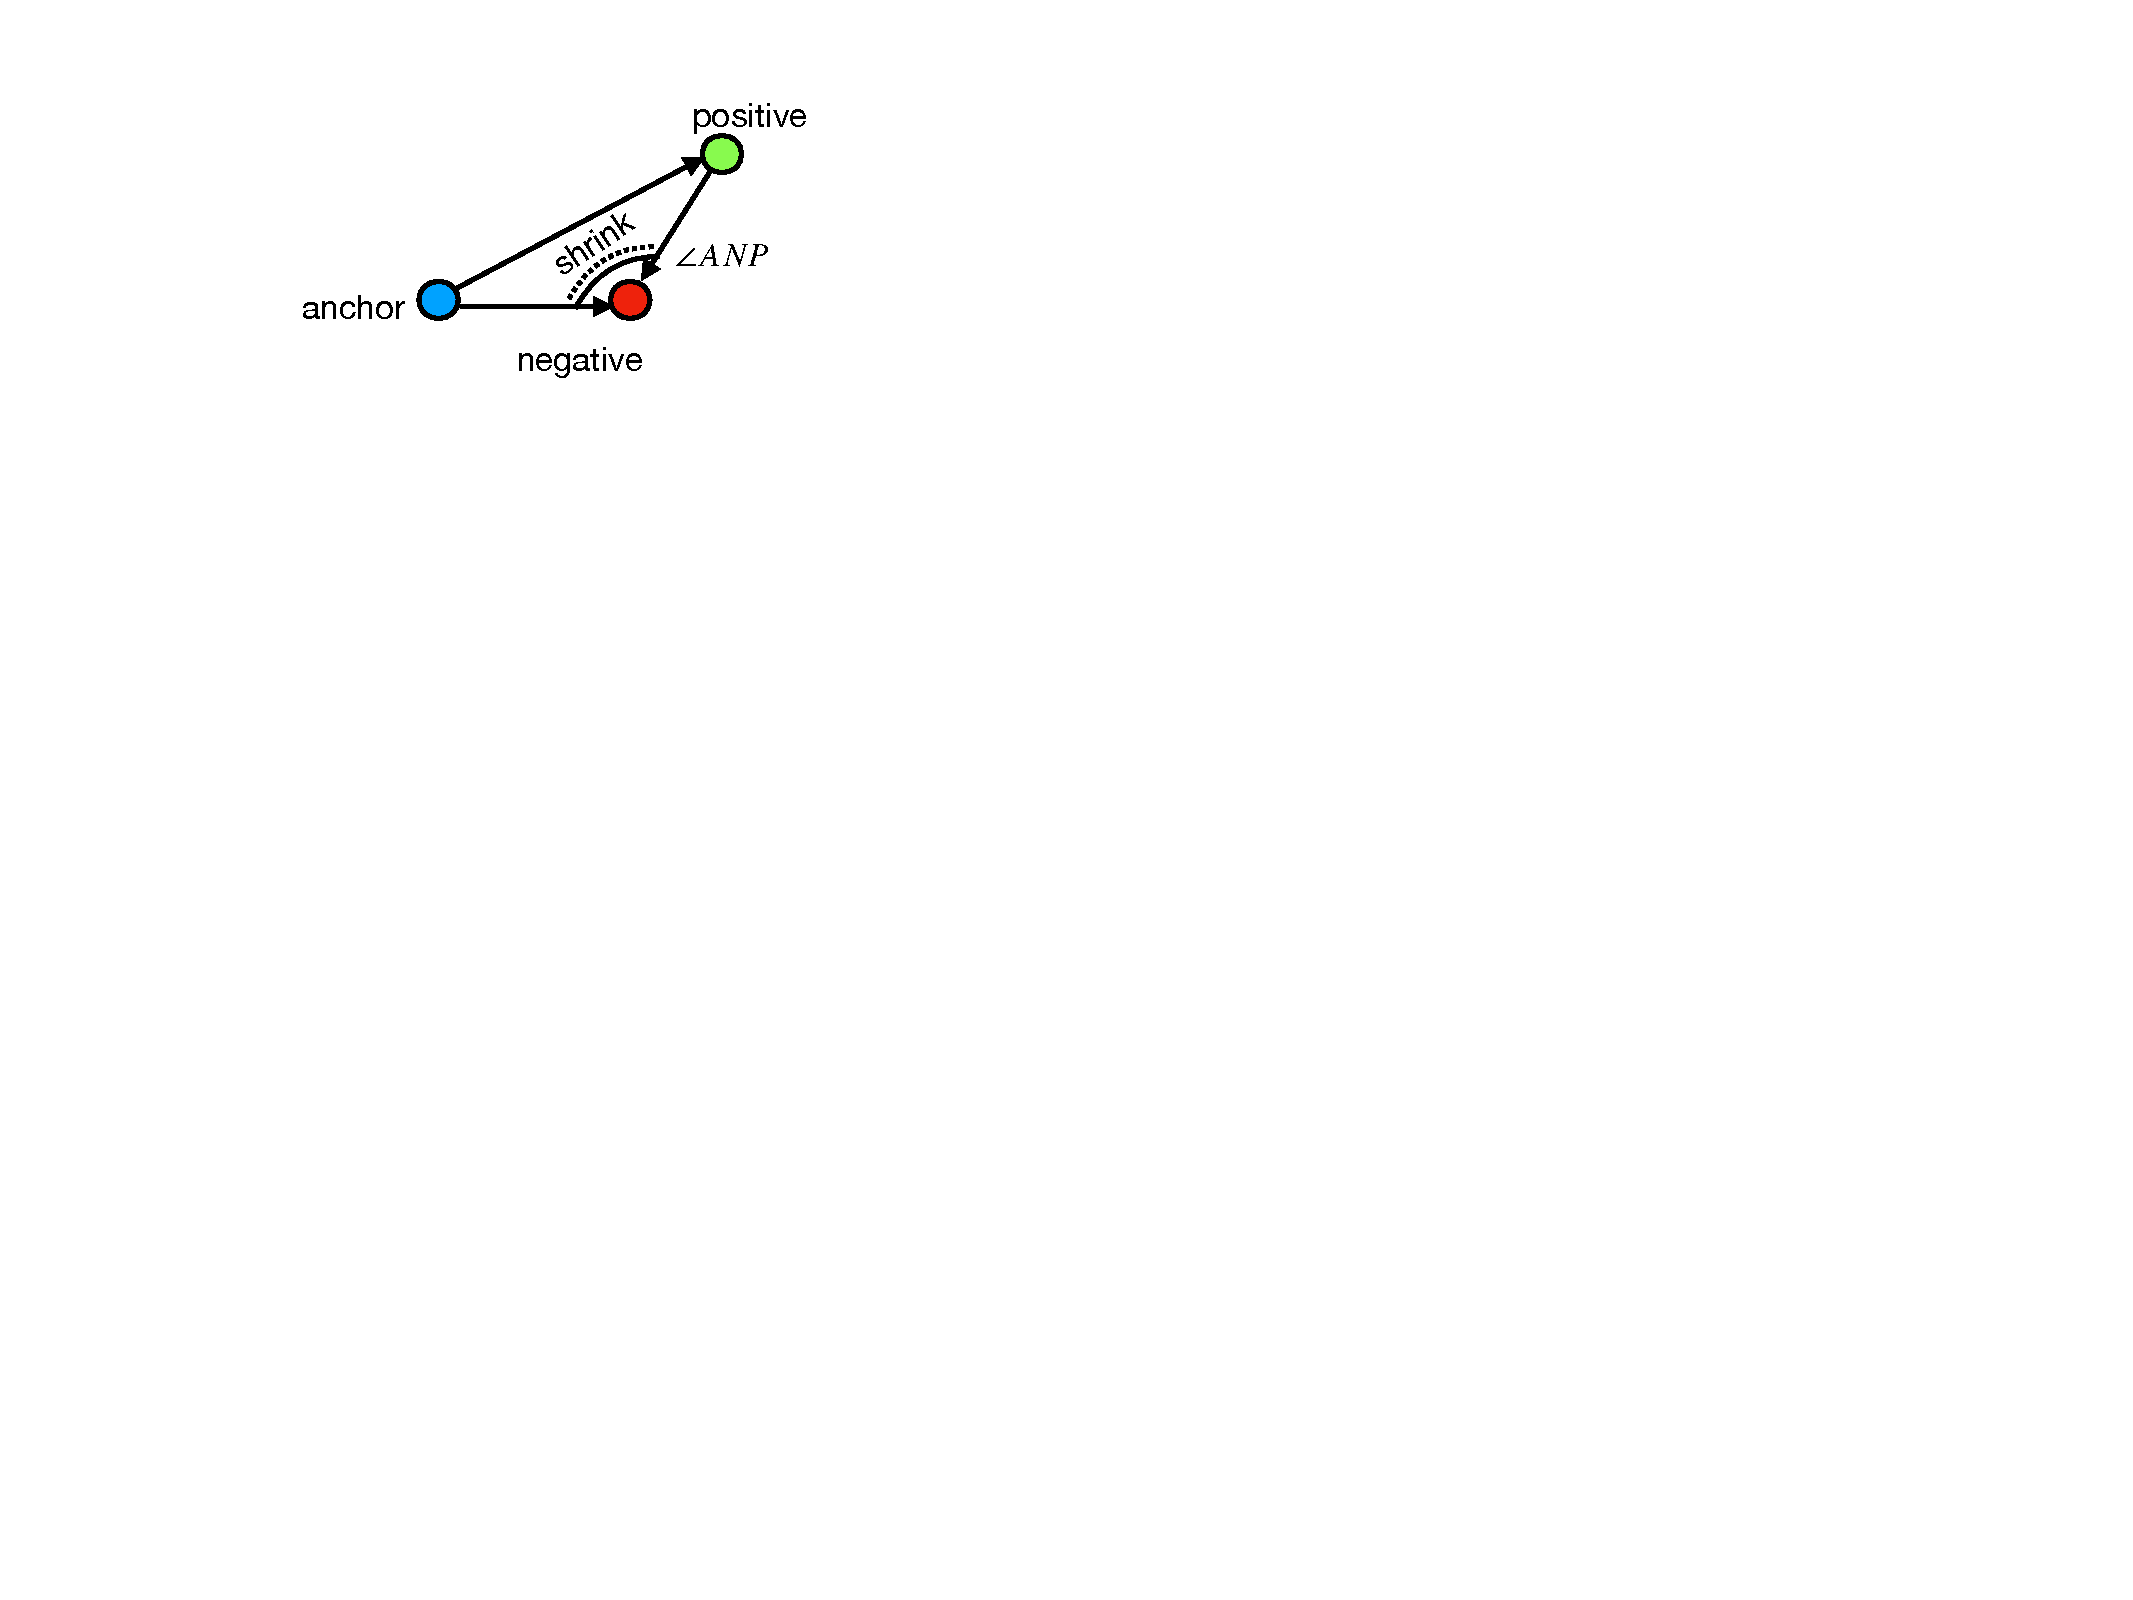
\includegraphics[width=.95\linewidth]{angular_loss}
        \caption{Angular loss}
        \label{angular_loss}
    \end{subfigure}
    \caption{Loss functions}
\end{figure}

\subsection{Triplet loss}

For face recognition, Schroff et al. \cite{DBLP:conf/cvpr/SchroffKP15}
propose a triplet loss function where the \textit{positive distances}
for each triplet $i$ in the set of $N$ triplets is separated from
\textit{negative distances} by a margin of $\alpha$, as shown in
Figure~\ref{schroff_loss} with the arrow pushing toward $\alpha$.  For
each of $N$ triples, $l_{triple}$ reflects the loss for a given triple
as follows: 
\begin{equation}
  l_{triple} =  \left[\|\bf{x_a} - \bf{x_p}\|^2 - \|\bf{x_a} -\bf{x_n}\|^2 + \alpha \right]_+
\label{schroff}
\end{equation}
where
\begin{equation}
 \left[.\right]_{+} = max(0, .)
\end{equation}
and the loss function that is minimized across all $N$ triples is given by
\begin{equation}
 L = \sum_{i}^{N} l_{triple}
\end{equation}
Note that in this formulation, it is assumed that embedding is normalized so $\|\bf{x} \| = 1$ because this normalization is robust across variations in illumination and contrast.  The value of $\alpha$ in the original work is a hyper-parameter that \cite{DBLP:conf/cvpr/SchroffKP15} was set to 0.2.

\subsection{Improved Loss}

 An improvement over the triplet loss function is proposed by
 \cite{DBLP:conf/cvpr/SchroffKP15} for the recognition of faces in
 videos \cite{Zhang:2016:DML:3088616.3088665}.  Conceptually, this
 function that we refer to as `improved loss' in the paper considers
 the distances from the \textit{positive} to the \textit{negative}, and tries to push that
 difference toward $\alpha$ as well as the distance from
 \textit{anchor} to the \textit{negative}.  We show this in
 Figure~\ref{modified_loss} with two push arrows.  In addition, it corrects the fact the  original triplet loss function has no constraints on how close the positive distance should be.  For instance, it is possible for the \textit{anchor} and \textit{positive} form a large cluster with a large intra-class distance. The equations that achieve these constraints are described below.  Equation~\ref{psi} tries to reduce intra-class distance by ensuring it is less than $\hat{\alpha}$.  Equation~\ref{phi} tries to maximize inter-class distance by ensuring that the distance from the \textit{anchor} and \textit{positive} to the negative are both taken into account.  Equation~\ref{improved_loss} balances inter-class constraints with intra-class constraints with the parameter $\lambda$. 

\begin{equation}
  \psi_{triple} = \|\bf{x_{a}} - \bf{x_{p}}\|^2 - \hat{\alpha}
\label{psi}
\end{equation}
\begin{equation}
  \phi_{triple} = \|\bf{x_{a}} - \bf{x_{p}}\|^2 - (\|\bf{x_{a}}- \bf{x_{n}}\|^2 + \|\bf{x_{p}} - \bf{x_{n}}\|^2) / 2  + \alpha
\label{phi}
\end{equation}
\begin{equation}
  l_{triple} = max(0, \phi) + \lambda * max(0, \psi)
\label{improved_loss}
\end{equation}
The parameter $\hat{\alpha}$ for equation~\ref{psi} is set to 0.1, and $\lambda$ is set to .02 in equation~\ref{improved_loss}, and $\alpha$ was set to 1 in the paper \cite{Zhang:2016:DML:3088616.3088665}.  As in Schroff et al. \cite{DBLP:conf/cvpr/SchroffKP15}, the embeddings are normalized to 1 although the actual paper does not make it clear.

\subsection{Angular Loss}

Wang et al. \cite{DBLP:journals/corr/abs-1708-01682} define a novel
angular loss function which is not based on pairwise distances, but
rather is based on the angles of the triangle formed by the
\textit{anchor}, \textit{positive} and the \textit{negative} triplet.
Conceptually, they point out that since the \textit{anchor} and the
\textit{positive} pairs belong to the same class, the angle formed by
the \textit{anchor}, \textit{negative}, and \textit{positive} elements
should be as small as possible within that triangle.  Their loss
function is an attempt to minimize this angle, as defined in the
equations below.  The rough idea is that moving the positive nearer
and the \textit{negative} further away each reduce the angle, which we
illustrate in Figure~\ref{angular_loss} with the angle to shrink.
\begin{equation}
\bf{x_{c}} = (\bf{x_{a}} + \bf{x_{p}}) / 2
\end{equation}
\begin{equation}
l_{triplet} = \left[[\bf{x_{a}} - \bf{x_{p}}\|^2 - 4 \tan^2 \alpha \|\bf{x_{n}} - \bf{x_{c}}\|^2 \right])_{+}
\end{equation}

\subsection{Adapted Loss}

The inspiration for adapting the original triplet loss is to separate the effect of the positive
and negative distances as much as possible.  Rather than subtracting
the negative distance from the positive one, we want to negate the
negative distance and then add the two.  To approximate this, we
subtract the negative distance from a margin, and use 0 instead if
that difference is negative.  We then combine the squared distances as
usual, as how in Figure~\ref{adapted}.

\begin{equation}
  l_{triple} =  \|\bf{x_a} - \bf{x_p}\|^2 + \left[ \alpha - \|\bf{x_a} -\bf{x_n}\| \right]_+^2
\label{adapted}
\end{equation}

\section{Triplet Selection}
As discussed earlier, deep metric learning for faces is a difficult problem for neural networks to learn because improper sample selection can make it difficult for the network to converge.  We describe a popular approach batch based approach from the face recognition literature first to contrast it with our mechanism for triplet selection.

\subsection{Batch Based Triple Selection}
\begin{figure}
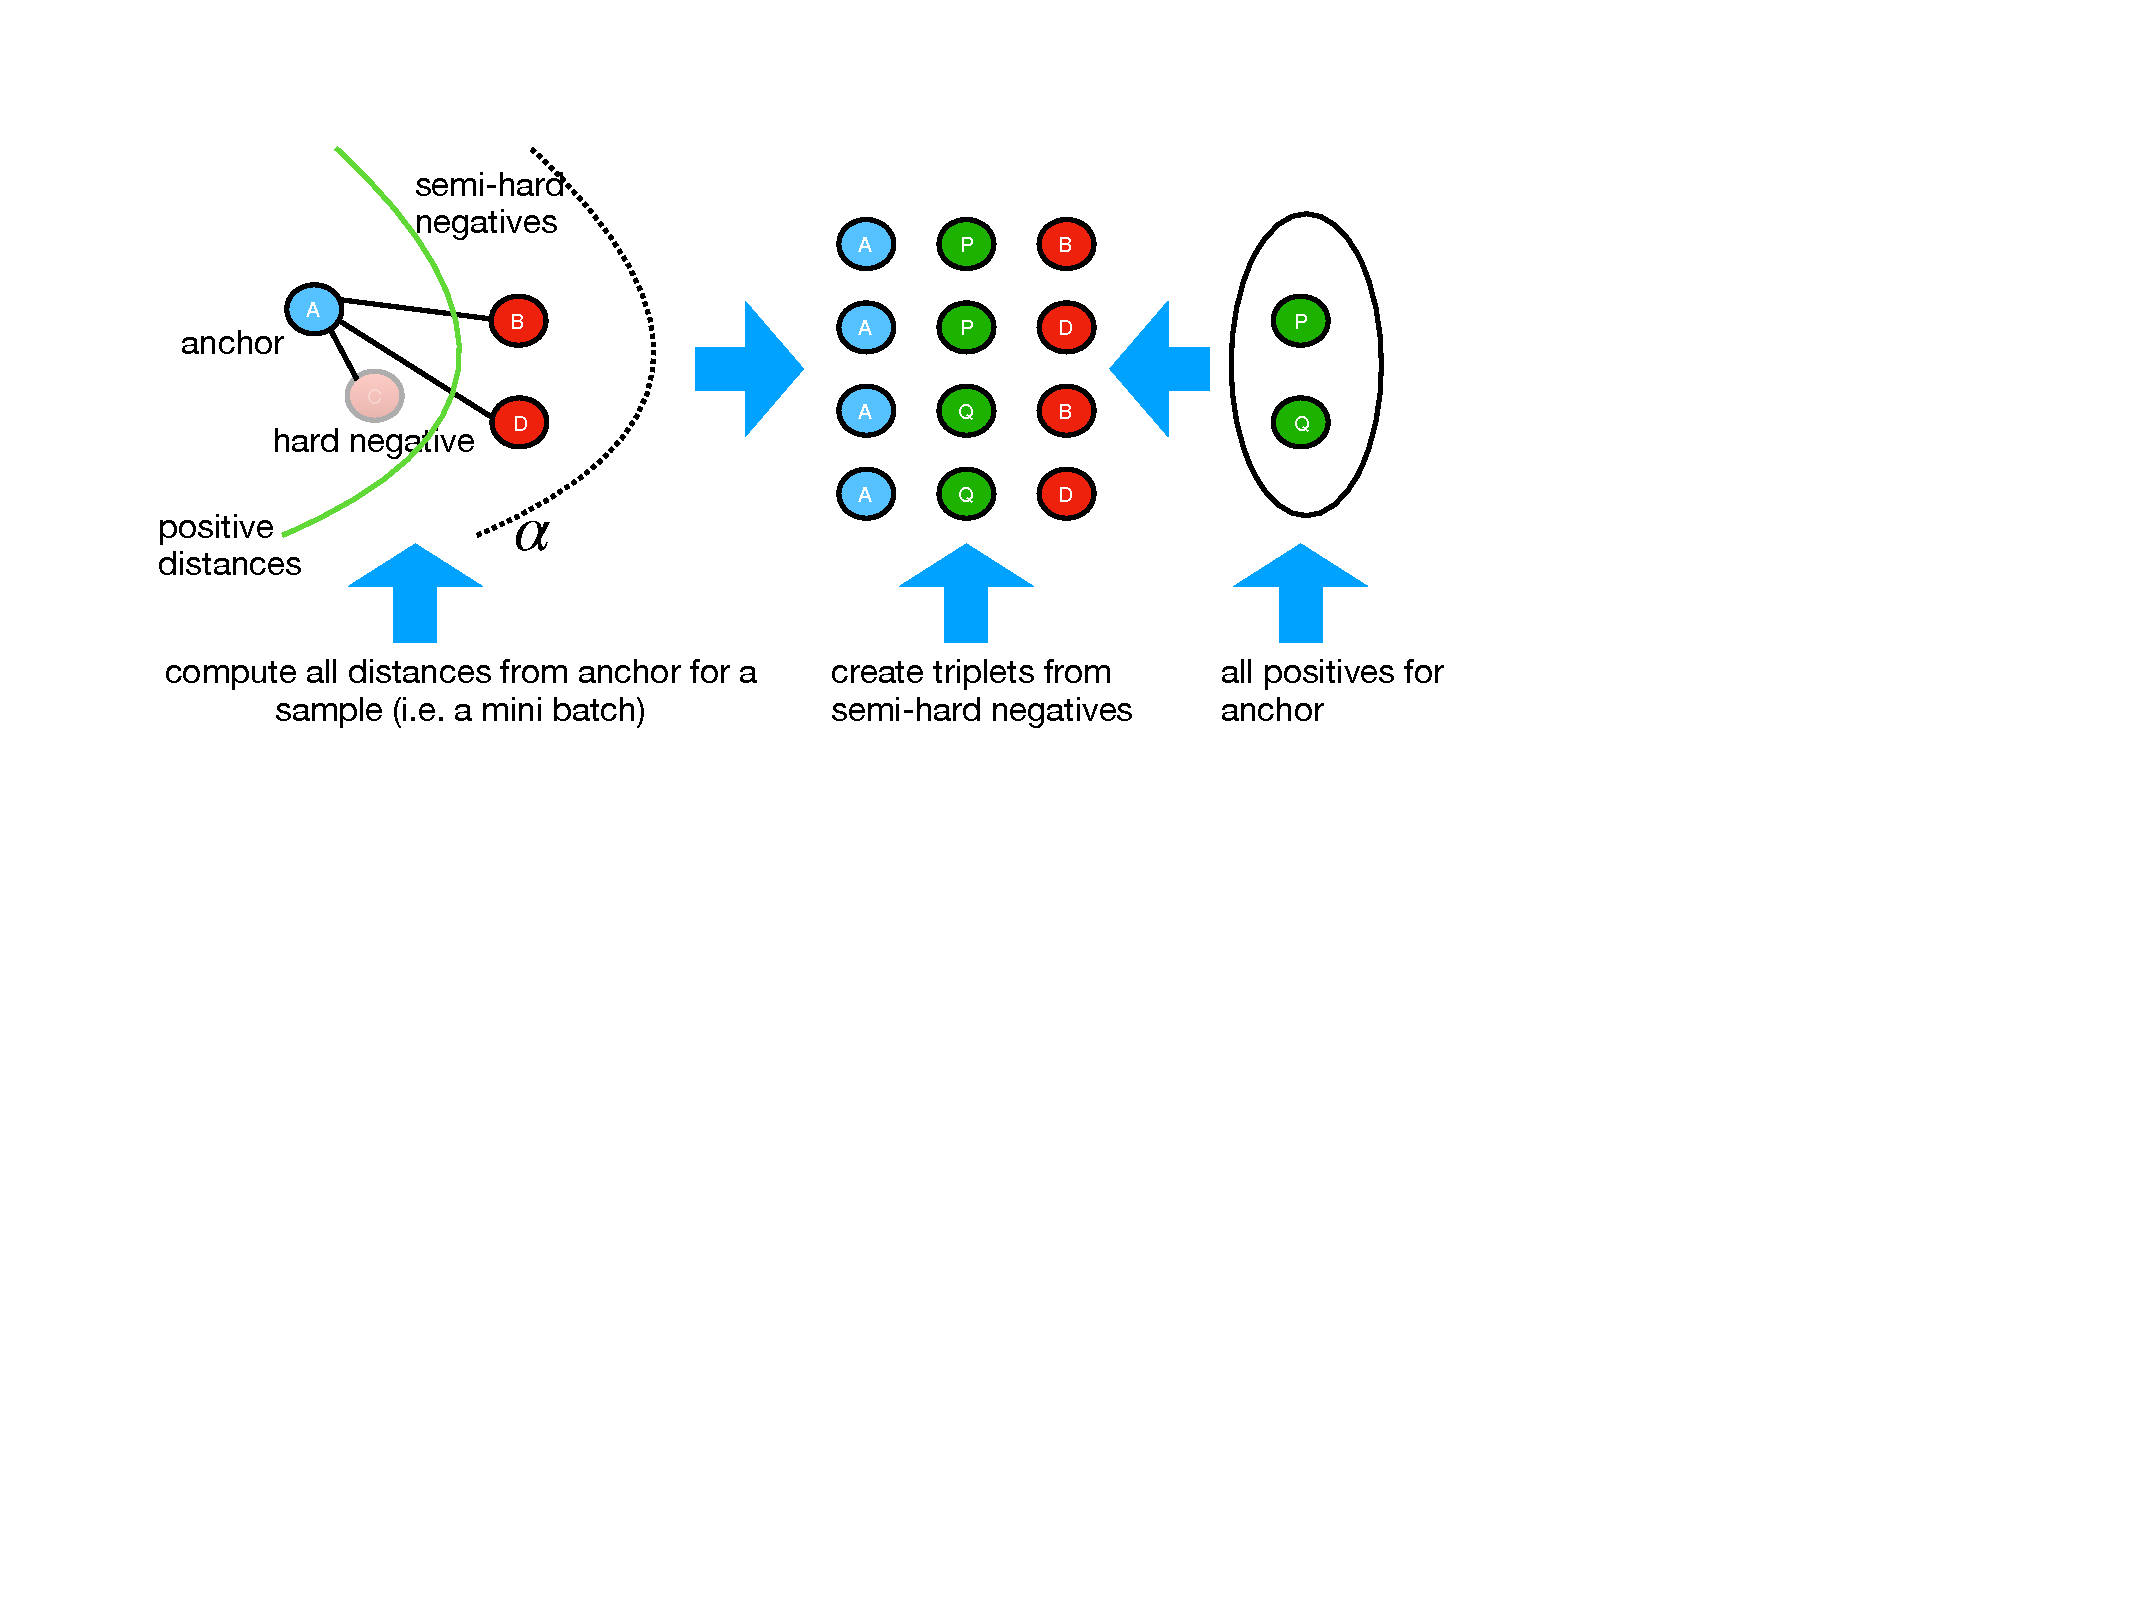
\includegraphics[width=1.0\linewidth]{triplet_selection}
\caption{Batch based triplet selection}
\label{triplet_selection}
\end{figure}

In Schroff et al.'s work~\cite{DBLP:conf/cvpr/SchroffKP15} they discuss a sample or mini-batch based triplet selection mechanism for training.  Conceptually, sampling the `right' triplets for fast network learning, as Schroff et al. point out requires sampling a set of \textit{hard positives} and a set of \textit{hard negatives}, where a hard positive is defined as $argmax^i \| x_{a} - x_{p}^i \|^2$, where $i$ ranges over all $x_p$ and a hard negative is defined as $argmin^i \| x_{a} - x{_n}^i \|^2$, where $i$ ranges over all $x_n$. 

However, it is infeasible to compute these values for the entire dataset.  Calculating hard positives is easy because the number of \textit{positives} is small normally.  Calculating hard negatives is not possible for all but small datasets.  As a result, the triplets can be generated either offline, for every n steps, or online, by selecting positive and negative exemplars within a batch of examples.  In Schroff et al.'s work, they focus on the online generation case.  

Figure~\ref{triplet_selection} shows the triplet selection mechanism used in their work.  In practice, instead of focusing on finding \textit{hard positives}, they instead pair every possible positive in the sample shown in the right panel in the figure with selected negatives, since the set of positives is usually quite small.  Furthermore, for negative examples, they try to select \textit{semi-hard negatives} instead of \textit{hard negatives}, where a \textit{semi-hard negative} has the property that $\|x_a - x_p \|^2 < \|x_a - x_n \|^2$.  As shown in the figure~\ref{triplet_selection} a \textit{semi-hard negative} is further from the \textit{anchor} than the \textit{positive}, but is not distant enough.  That is, the loss function still needs to move it closer to the margin $\alpha$ that is used in the triplet-loss function.  Schroff et al. further argue selecting \textit{hard negatives} such as $C$ in the figure may in fact lead to bad local minima early on in training, and lead to a collapsed model where the function always learns to return a value of 0, regardless of the pair being considered.

\subsection{Metric Based Triplet Selection}
Although the computation of there is $argmax^i \| x_{a} - x_{p}^i \|^2$ and $argmin^i \| x_{a} - x{_n}^i \|^2$ is infeasible because it involves quadratic comparisons within a dataset, we observe that the use of approximate nearest neighbor (ANN) indexes can actually make this problem tractable for the selection of triples.  

Approximate nearest neighbor indexes are highly efficient methods for selecting the top-K neighbors of a given vector by Euclidean distance, cosine similarity or other distance metrics.  They are based on space partitioning algorithms, such as \textit{k-d trees}, where the vector space is iteratively bisected into two disjoint regions.  Finding the nearest neighbors of a vector involves traversal of the tree to a leaf by evaluating the queried vector at each split point in the tree.  Depending on the position of the vector within the space bounded by a split point, it may need to traverse both points at a split node.  However, large portions of the tree (and hence most vectors in the dataset) never get compared to the queried vector.  The average complexity to query the vectors of a neighbor is $O(log N)$ where N is the number of vectors in the dataset.  Implementations exist now for fast, memory-efficient ANN indexes that scale up to a billion vectors \cite{JDH17} using techniques to compress vectors in memory efficiently.  In our work, we used the Annoy ANN implementation \cite{annoy_git} in our work which is based on the refinements to \textit{k-d trees} ideas described in \cite{ann_paper}.

\begin{figure}
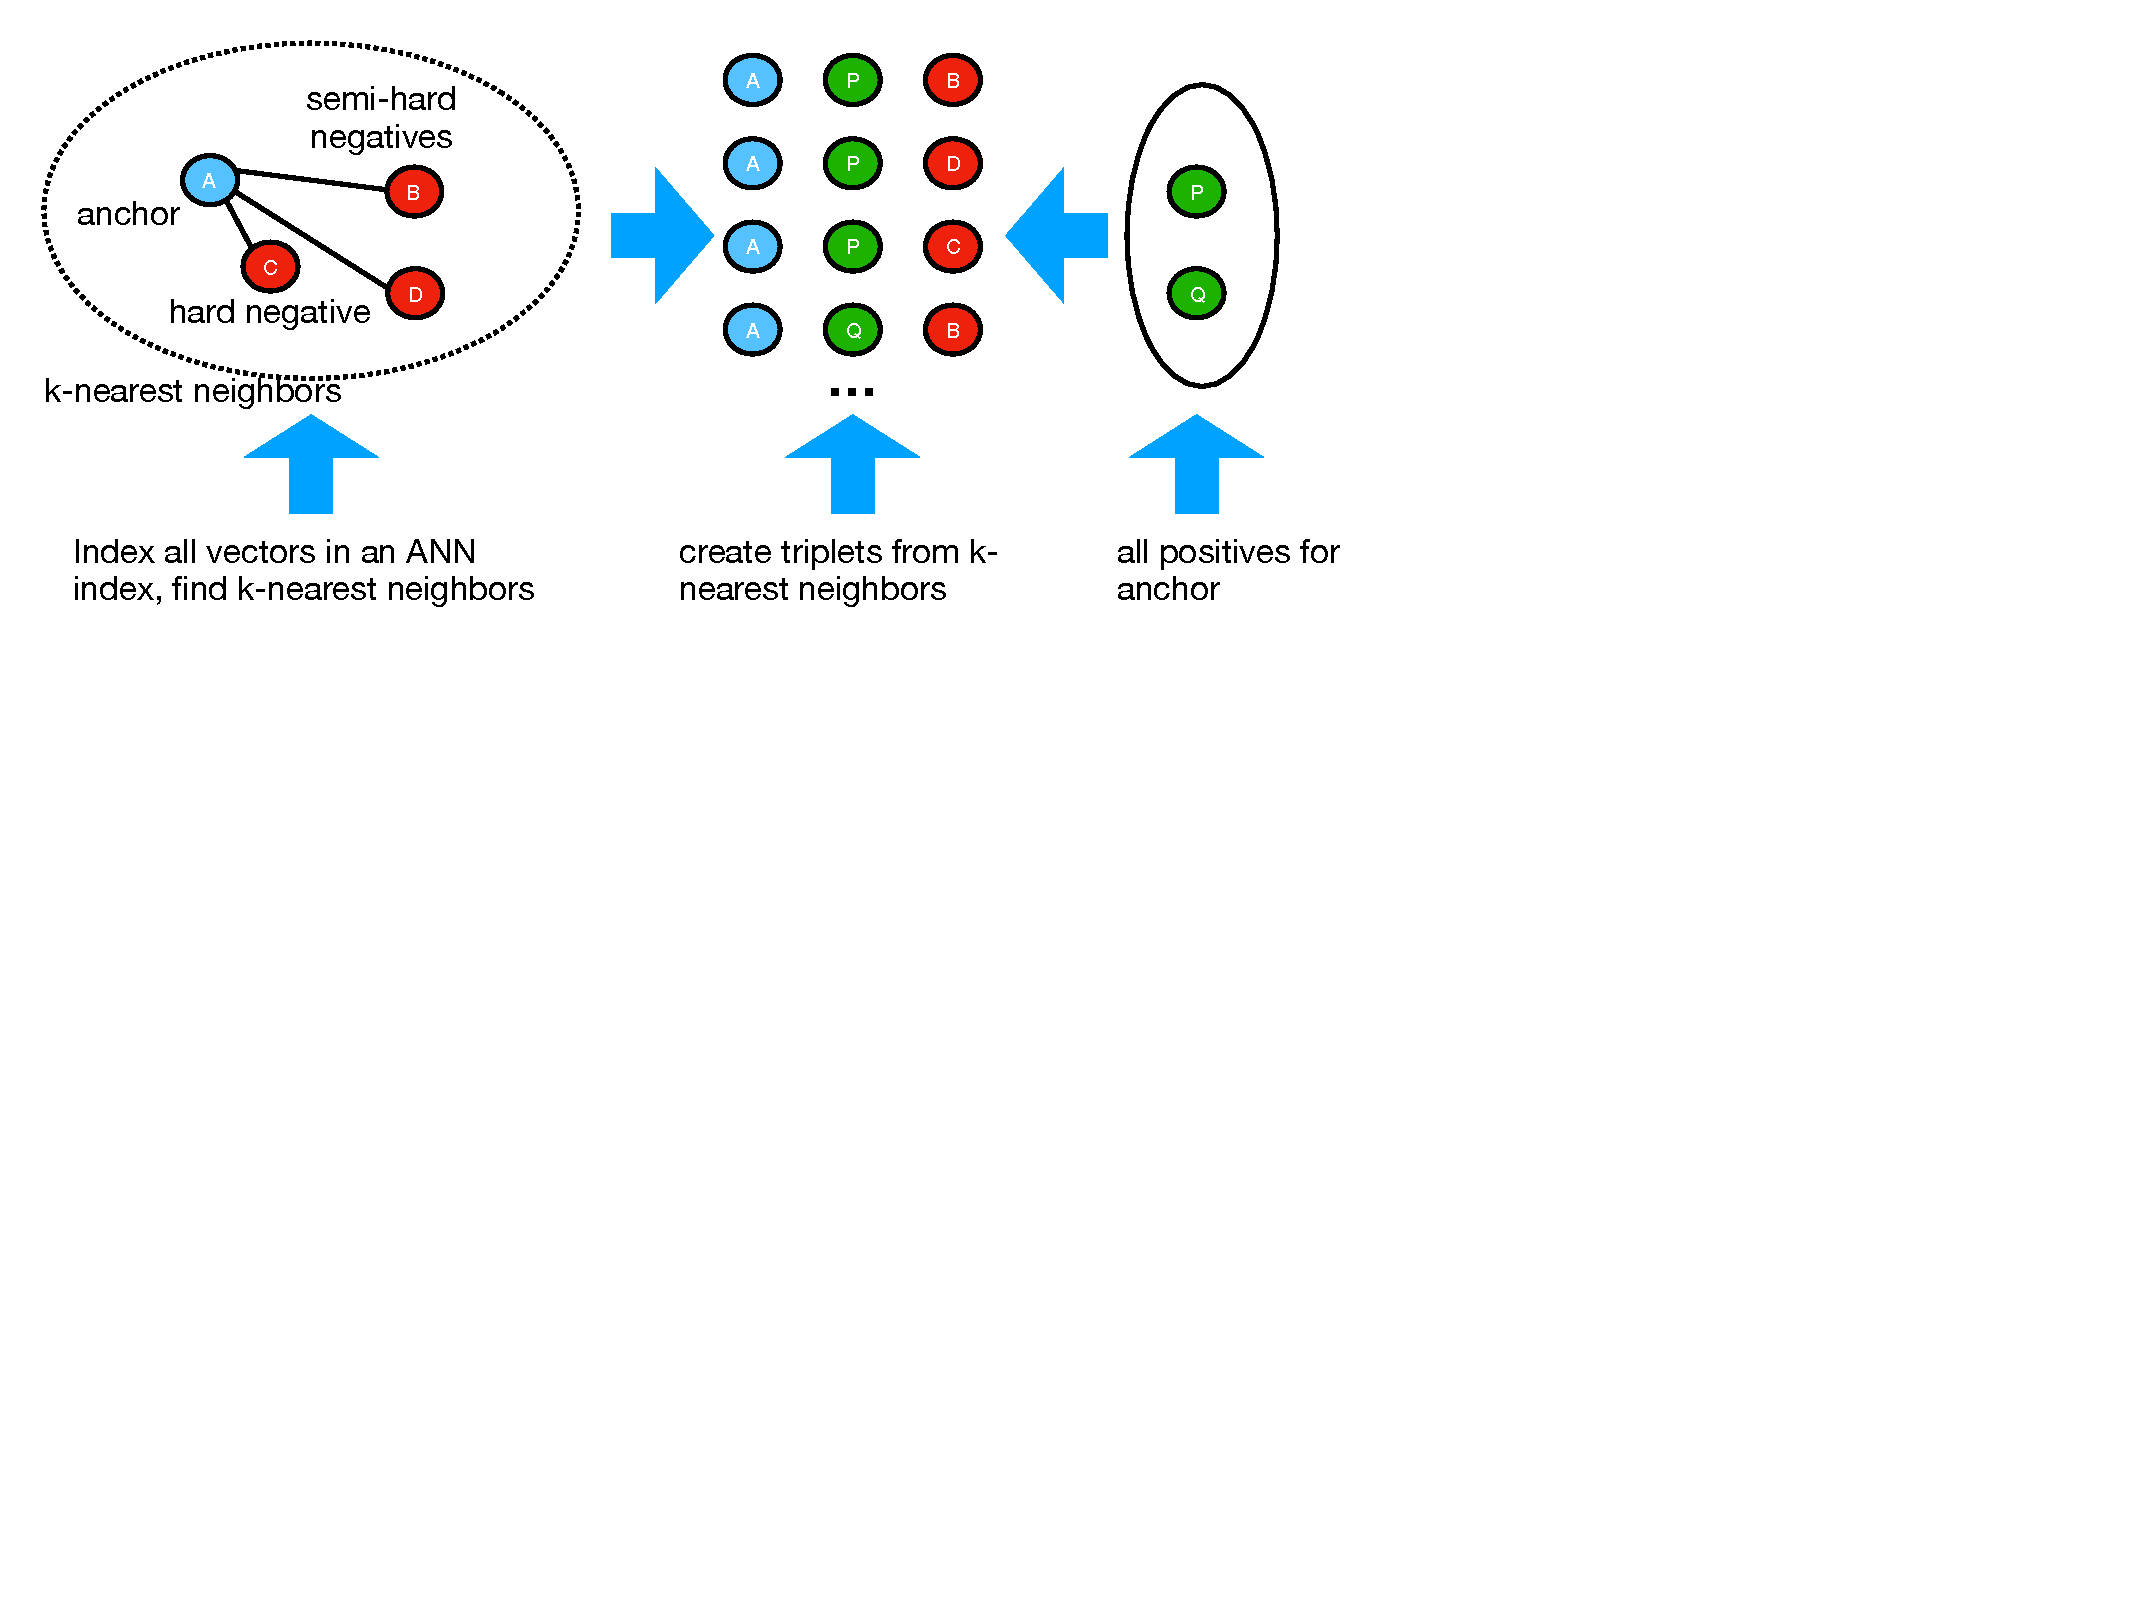
\includegraphics[width=1.0\linewidth]{ANN_selection}
\caption{ANN based triplet selection}
\label{ANN_selection}
\end{figure}

Assuming one has the entire dataset indexed in an ANN index, the problem of triplet selection can be simplified by asking the ANN index for the top k-nearest neighbors of an \textit{anchor}, where k is given by the number of triplets that one desires to generate for each anchor.  As in earlier work, selection of \textit{hard positives} is not really relevant because all positive data should be used to teach the network the right function.  Selection of negatives is the set of all nearest neighbors that are \textit{negatives}.  There is no explicit attempt to filter out\textit{hard negatives} in the approach.  The overall idea is that the set of negatives that appear in the nearest neighbor set at input are in fact the most important elements for the network to learn to discriminate from positives for a join.  Focusing on these elements, regardless of whether they are \textit{hard} or \textit{semi-hard} should lead to better discrimination for joins.  An ANN-based strategy also provides an important baseline to assess what if any learning was performed by the neural network in mapping input vectors to a different space.

